\documentclass[11pt,a4paper]{article}
\usepackage[margin=2cm,top=1.8cm,bottom=1.8cm]{geometry}
% Préambule commun aux deux documents
\usepackage[T1]{fontenc}
\usepackage[french]{babel}
\usepackage{lmodern}
\usepackage{amsmath,amssymb}
\usepackage{graphicx,xcolor,booktabs,array,tabularx,longtable}
\usepackage{tikz}
\usetikzlibrary{positioning,arrows.meta,shapes.geometric,calc,fit,backgrounds,decorations.pathreplacing}
\usepackage{fancyhdr,enumitem,microtype}
\usepackage[colorlinks=true,linkcolor=aegis,urlcolor=aegis,citecolor=aegis]{hyperref}
\usepackage{caption}
\usepackage{listings}

\definecolor{aegis}{RGB}{14,116,144}
\definecolor{aegisfonce}{RGB}{11,18,32}
\definecolor{grisfond}{RGB}{247,248,250}
\definecolor{grisligne}{RGB}{216,220,226}
\definecolor{gristexte}{RGB}{91,97,107}
\definecolor{vertok}{RGB}{26,127,75}
\definecolor{orangepartiel}{RGB}{178,106,5}
\definecolor{rougeko}{RGB}{198,40,40}

\captionsetup{font=small,labelfont={bf,color=aegis}}
\setlist[itemize]{leftmargin=1.2em,itemsep=1pt,topsep=2pt,parsep=0pt}
\setlist[enumerate]{leftmargin=1.4em,itemsep=1pt,topsep=2pt,parsep=0pt}

\lstset{
  basicstyle=\ttfamily\scriptsize,
  backgroundcolor=\color{grisfond},
  frame=single, rulecolor=\color{grisligne},
  breaklines=true, showstringspaces=false,
  keywordstyle=\color{aegis}\bfseries,
  commentstyle=\color{gristexte}\itshape,
  numberstyle=\tiny\color{gristexte},
  xleftmargin=4pt, framexleftmargin=4pt, aboveskip=6pt, belowskip=6pt,
  literate={é}{{\'e}}1 {è}{{\`e}}1 {à}{{\`a}}1 {ç}{{\c c}}1 {ê}{{\^e}}1 {û}{{\^u}}1 {î}{{\^i}}1 {ô}{{\^o}}1 {É}{{\'E}}1 {—}{{---}}1 {’}{{'}}1 {«}{{<<}}1 {»}{{>>}}1 {·}{{\textperiodcentered}}1
}

% Marqueurs d'état
\newcommand{\ok}{\textcolor{vertok}{\textbf{Atteint}}}
\newcommand{\partiel}{\textcolor{orangepartiel}{\textbf{Partiel}}}
\newcommand{\absent}{\textcolor{rougeko}{\textbf{Non traité}}}
\newcommand{\plus}{\textcolor{aegis}{\textbf{Au-delà}}}

% Mesure mise en avant dans le fil du texte
\newcommand{\mesure}[1]{\textcolor{aegis}{\textbf{#1}}}

% Les paragraphes techniques enchaînent de longues suites en \texttt{} que TeX
% ne peut pas couper : sans marge de man\oe{}uvre, elles débordent dans la marge.
\emergencystretch=2em
\hbadness=4000


\pagestyle{fancy}\fancyhf{}
\renewcommand{\headrulewidth}{0.4pt}
\fancyhead[L]{\small\textcolor{gristexte}{AEGIS Mini-SOC --- Rapport de projet}}
\fancyhead[R]{\small\textcolor{gristexte}{Détection d'intrusion réseau}}
\fancyfoot[C]{\small\thepage\ / \pageref{LastPage}}
\usepackage{lastpage}

\setlength{\parskip}{3pt}
\setlength{\parindent}{0pt}

\begin{document}

%================================================================ TITRE
\begin{center}
{\LARGE\bfseries AEGIS Mini-SOC}\\[2pt]
{\large Détection d'intrusion réseau par apprentissage automatique,\\et poste de travail d'analyste}\\[6pt]
{\small Mohamed Aziz BAOUEB}\\[2pt]
{\small\textcolor{gristexte}{Code source : \url{https://github.com/aziz3r/aegis-mini-soc}}}
\end{center}
\vspace{-4pt}
\rule{\linewidth}{0.8pt}

%================================================================ 1
\section{Introduction}

Un système de détection d'intrusion classique fonctionne par \textbf{signatures} : il reconnaît une
attaque parce qu'il en a déjà rencontré l'empreinte exacte. Ce modèle est efficace sur le connu et
aveugle sur le reste ; une variation mineure suffit souvent à le contourner.

AEGIS adopte l'approche \textbf{comportementale} : apprendre ce qu'est le trafic normal d'un réseau,
puis signaler ce qui s'en écarte. Ce choix permet de détecter une attaque jamais vue, mais il
déplace la difficulté vers trois problèmes que ce projet traite explicitement.

\textbf{Un score d'anomalie n'a pas de sens en soi.} Savoir qu'un flux obtient 0,87 ne dit rien tant
qu'on ignore à quoi le comparer. Le score est donc passé par la fonction de répartition empirique du
trafic bénin : 0,97 signifie alors exactement \og{}plus inhabituel que 97\% du trafic normal
connu\fg{}, et un seuil posé sur ce nombre devient interprétable.

\textbf{Un seuil unique ne peut convenir à toutes les machines.} Un serveur de sauvegarde qui
contacte douze hôtes à trois heures du matin et le poste de l'accueil n'ont pas la même normale.
Chaque hôte dérive donc son seuil du quantile de son propre historique, au-dessus d'un plancher
commun.

\textbf{Un détecteur sensible noie l'analyste.} Une inondation produit des milliers d'alertes par
minute ; les présenter une par une est le mécanisme par lequel un centre opérationnel cesse de lire
ses propres alertes. Les alertes sont donc corrélées en incidents, regroupés selon la forme de
l'attaque.

Le projet comprend la chaîne complète : capture et assemblage de flux, extraction de 52
caractéristiques, modèle à deux étages, seuils adaptatifs, corrélation, et une interface web de
triage en huit écrans. Il est accompagné d'un protocole de mesure et de résultats chiffrés.

%================================================================ 2
\section{Aperçu de l'architecture}

\begin{figure}[h]\centering
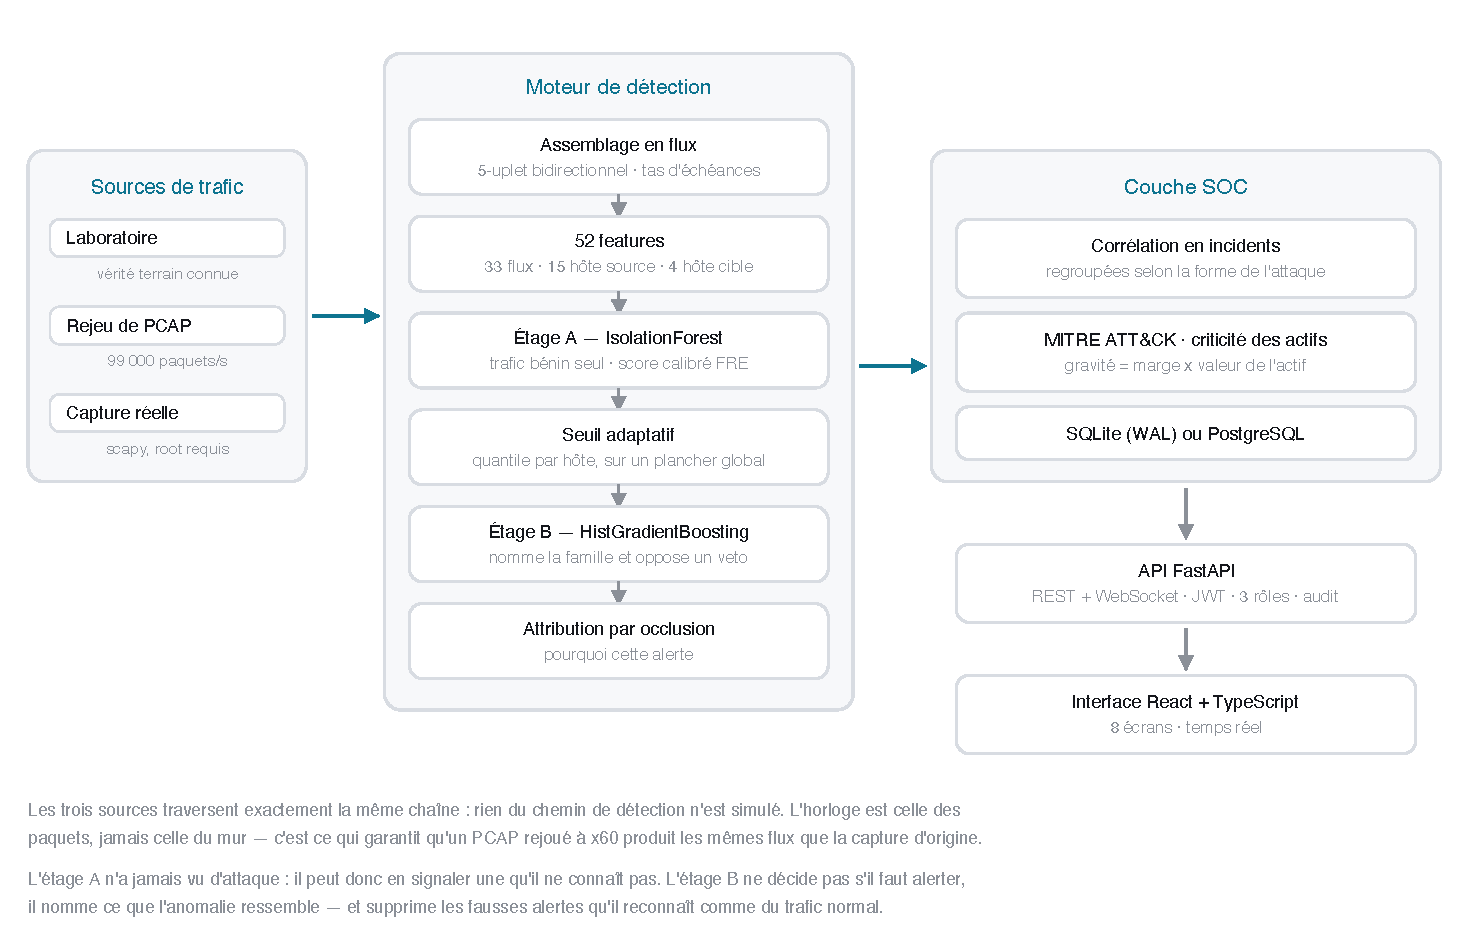
\includegraphics[width=0.98\linewidth]{../docs/architecture.pdf}
\caption{Des paquets aux incidents. Les trois sources traversent la même chaîne.}
\end{figure}

Le trafic peut provenir de trois sources --- un réseau de laboratoire synthétique, un fichier PCAP
rejoué, ou une interface réelle --- et traverse exactement le même moteur. Rien du chemin de
détection n'est simulé : seule la provenance du trafic change.

L'horloge utilisée est celle des \textbf{paquets}, jamais celle du mur. C'est cette décision qui
garantit qu'une capture rejouée à soixante fois la vitesse réelle produit les mêmes flux que la
capture d'origine, et donc que toute mesure faite sur fichier décrit bien le système déployé.

%================================================================ 3
\section{Le moteur de détection}

\subsection*{Assemblage en flux}

Les paquets sont regroupés en flux bidirectionnels identifiés par leur 5-uplet canonique. Un flux
est exporté lorsque la connexion se termine (RST, ou FIN des deux côtés), après quinze secondes
d'inactivité, ou après deux minutes s'il reste ouvert --- un téléchargement long est ainsi exporté
par tranches plutôt que de rester invisible.

Une tentative de connexion restée \textbf{sans réponse} fait exception : elle est exportée après
trois secondes. Un SYN sans réponse est déjà une observation complète, plus rien n'arrivera ;
conserver le flux pendant le délai d'inactivité complet ajoutait quinze secondes à la détection de
chaque balayage et de chaque inondation, les deux attaques composées presque entièrement de SYN sans
réponse. Cette seule modification a ramené la latence médiane de détection de seize à trois
secondes.

L'expiration des flux repose sur deux tas d'échéances paresseux. La version initiale parcourait tous
les flux actifs à chaque paquet, un coût proportionnel au nombre de connexions ouvertes --- qui
s'effondrait précisément pendant une inondation ou un slowloris, dont le principe même est d'ouvrir
des milliers de connexions simultanées. Le débit est passé de \mesure{12 000} à \mesure{33 000
paquets par seconde}, et l'équivalence avec le parcours naïf est vérifiée par un test sur quatre
minutes de trafic mixte.

\subsection*{Cinquante-deux caractéristiques}

\begin{table}[h]\centering\small
\begin{tabularx}{\linewidth}{@{}l r X@{}}
\toprule
\textbf{Groupe} & \textbf{Nb} & \textbf{Exemples} \\
\midrule
Intrinsèques au flux & 33 & durée, paquets/s, octets/s, ratio aller/retour, moyenne et écart-type des
tailles, intervalles entre paquets, compteurs de drapeaux TCP, entropie de la charge utile \\
Comportement de la source & 15 & destinations et ports distincts sur 10 et 60 secondes, SYN/s sans
établissement, part de connexions échouées, ratio sortant/entrant, régularité de type balise \\
Comportement de la cible & 4 & flux reçus, sources distinctes, SYN/s non établis, part de connexions
échouées \\
\bottomrule
\end{tabularx}
\caption{Les trois familles de caractéristiques.}
\end{table}

Les quatre dernières méritent d'exister : une inondation dont les adresses sources sont usurpées est
\textbf{invisible côté source}, puisque chaque adresse falsifiée n'émet qu'un seul paquet. Seule
l'agrégation sur la victime la rend détectable.

Le numéro de port de destination brut est \textbf{volontairement exclu}. Un modèle à arbres
mémoriserait les ports du laboratoire et afficherait d'excellents scores sans rapport avec sa
capacité à généraliser ; seules les propriétés structurelles du port sont conservées.

\subsection*{Deux étages qui ne font pas le même métier}

\begin{table}[h]\centering\small
\begin{tabularx}{\linewidth}{@{}l X X@{}}
\toprule
 & \textbf{Étage A} & \textbf{Étage B} \\
\midrule
Algorithme & IsolationForest, 220 arbres & HistGradientBoosting, 300 itérations \\
Supervision & \textbf{aucune} --- trafic bénin seul & supervisée, 10 classes \\
Rôle & décider s'il faut alerter & nommer la famille, et opposer un veto \\
Sortie & score dans $[0,1)$, percentile du trafic normal & famille et confiance \\
Entraînement & 22\,295 flux bénins & 19\,397 flux, plafonnés par classe \\
\bottomrule
\end{tabularx}
\caption{Répartition des rôles entre les deux étages.}
\end{table}

L'étage A n'ayant jamais vu d'attaque, il peut en signaler une qu'il ne connaît pas : c'est la
propriété qui justifie l'approche comportementale. L'étage B, lui, ne décide pas s'il faut alerter ;
il nomme ce que l'anomalie ressemble, et refuse de nommer en dessous d'un seuil de confiance ---
une étiquette fausse mais assurée est plus nuisible à un analyste qu'une absence d'étiquette.

\subsection*{La cascade}

\begin{figure}[h]\centering
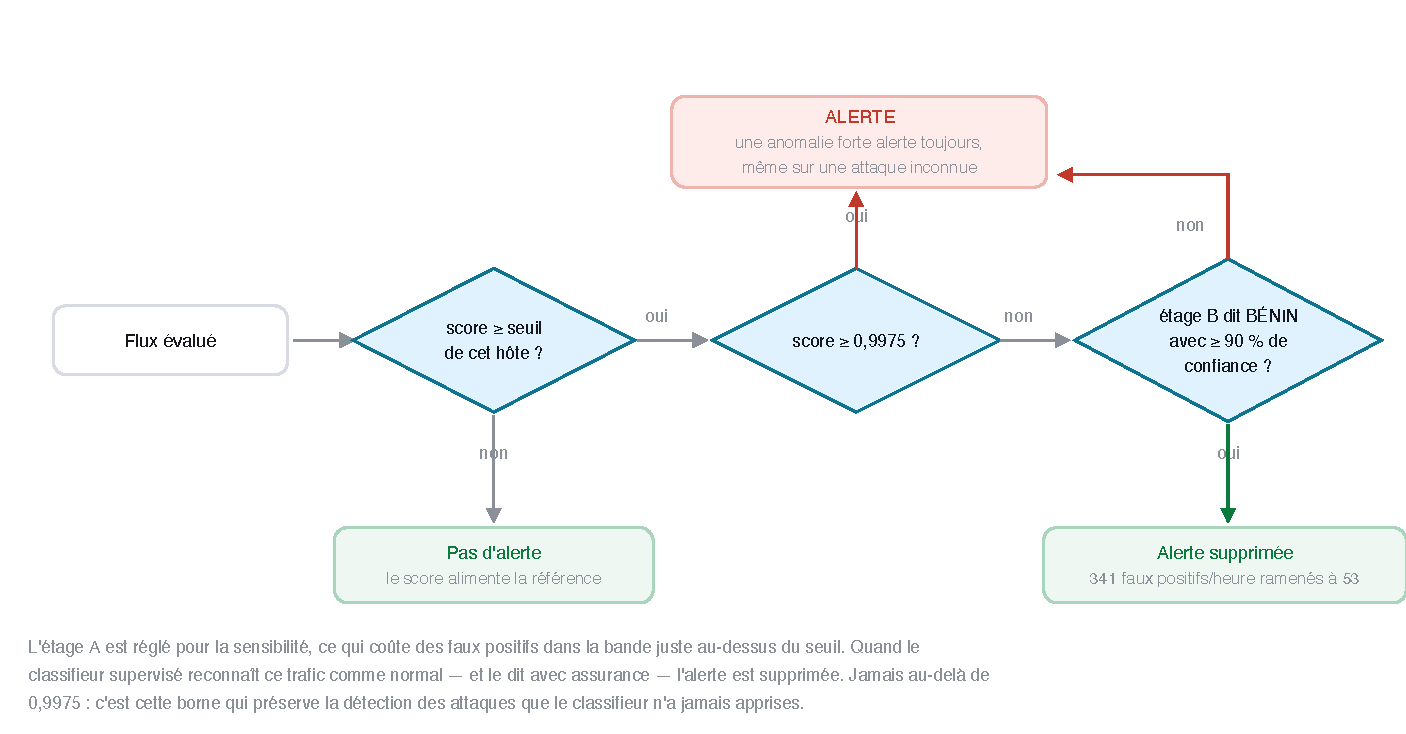
\includegraphics[width=0.96\linewidth]{../docs/cascade.pdf}
\caption{La décision d'alerter. L'étage B peut opposer son veto, mais jamais sur une anomalie forte.}
\end{figure}

L'étage A est réglé pour la sensibilité, ce qui coûte des faux positifs dans la bande située juste
au-dessus du seuil. Or l'étage B reconnaissait déjà ce trafic comme normal --- son avis était
simplement ignoré, puisqu'il n'intervenait qu'après la décision d'alerter.

Désormais, lorsque l'étage A signale un flux marginal que l'étage B reconnaît comme normal avec au
moins 90\% de confiance, l'alerte est supprimée. Jamais au-dessus de 0,9975 : au-delà de cette
borne, une anomalie forte alerte toujours, quoi qu'en dise le classifieur. C'est précisément ce qui
préserve la détection des attaques jamais apprises.

Effet mesuré : \mesure{341 faux positifs par heure ramenés à 53}, au prix de 0,6 point de rappel sur
les variantes furtives.

\subsection*{Un seuil par hôte}

\begin{figure}[h]\centering
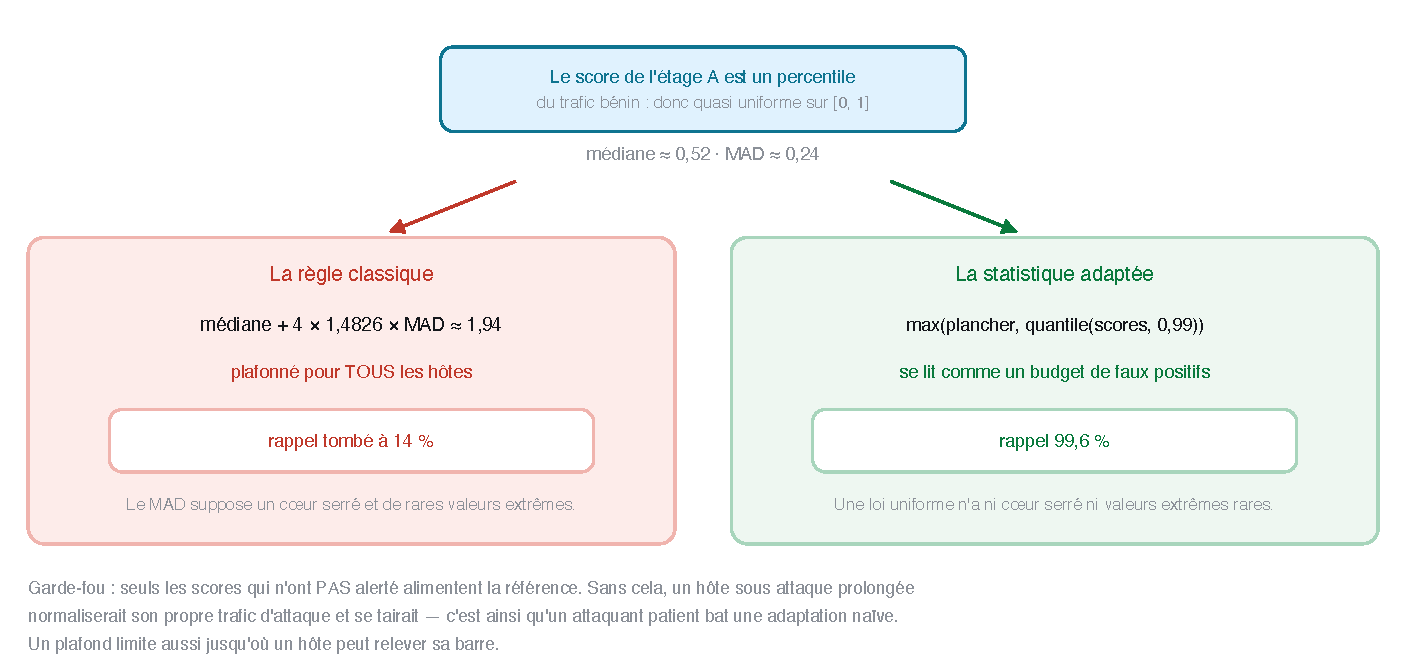
\includegraphics[width=0.96\linewidth]{../docs/seuil.pdf}
\caption{Pourquoi un quantile et non la règle robuste classique.}
\end{figure}

La première implémentation utilisait \texttt{médiane + k·MAD}, la règle robuste de manuel. Mesurée,
elle a fait tomber le rappel à \mesure{14\%}.

L'explication tient en une observation : les scores de l'étage A étant déjà des percentiles, ils
sont quasi uniformes sur le trafic normal. La médiane vaut environ 0,52, l'écart absolu médian 0,24,
et $0{,}52 + 4 \times 1{,}4826 \times 0{,}24 \approx 1{,}94$ saturait au plafond pour \emph{tous}
les hôtes. L'écart absolu médian suppose une distribution à c\oe{}ur serré avec de rares valeurs
extrêmes ; une loi uniforme n'a ni l'un ni l'autre.

Dans un espace de percentiles, la statistique pertinente est un quantile des scores de l'hôte, et
elle se lit directement comme un budget de faux positifs. Deux garde-fous l'accompagnent : seuls les
scores n'ayant pas déclenché d'alerte alimentent la référence --- sans quoi un hôte sous attaque
prolongée normaliserait son propre trafic d'attaque et se tairait --- et un plafond limite jusqu'où
un hôte peut relever sa propre barre.

%================================================================ 4
\section{De l'alerte à l'incident}

\begin{figure}[h]\centering
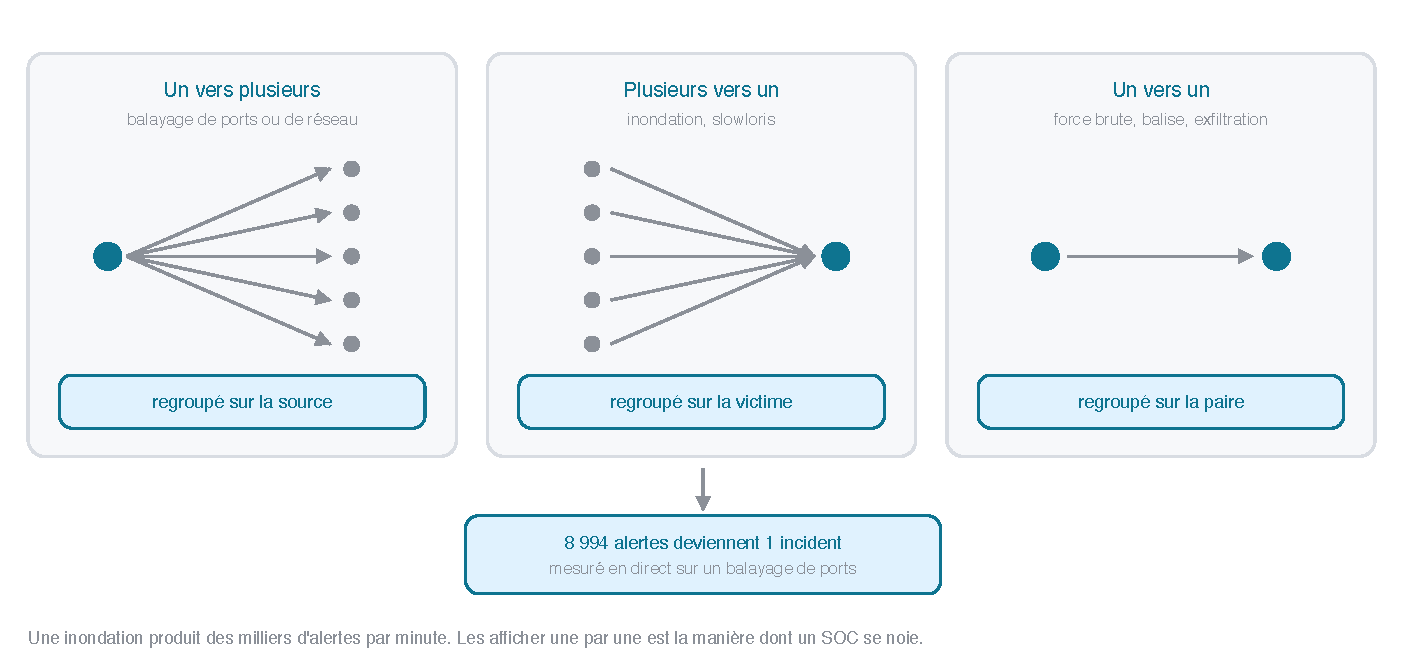
\includegraphics[width=0.96\linewidth]{../docs/correlation.pdf}
\caption{La clé de regroupement suit la forme de l'attaque.}
\end{figure}

La clé de regroupement dépend de la forme de l'attaque : un balayage se regroupe sur sa source, une
inondation sur sa victime, une force brute ou une balise sur la paire. Mesuré en fonctionnement :
\mesure{8\,994 alertes deviennent un seul incident}.

La gravité n'est pas le score. C'est la marge au-dessus du seuil \emph{de cet hôte}, pondérée par la
criticité de l'actif visé et par la confiance du classifieur. Un balayage de ports contre le serveur
de base de données passe donc devant un balayage plus bruyant contre une imprimante.

Chaque incident porte enfin sa correspondance MITRE ATT\&CK et une marche à suivre rédigée pour un
analyste, ainsi que l'explication de son déclenchement : chaque caractéristique est remplacée tour à
tour par sa valeur médiane sur le trafic normal et le flux réévalué ; la chute du score mesure sa
contribution.

%================================================================ 5
\section{L'interface}

\begin{figure}[h]\centering
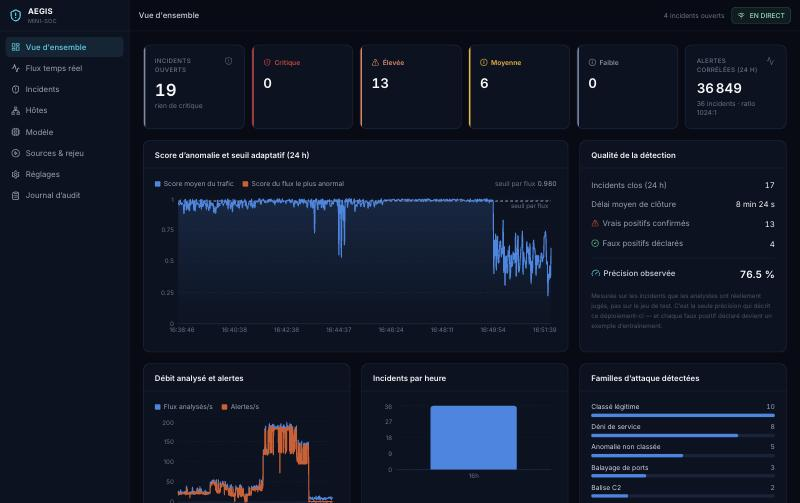
\includegraphics[width=0.98\linewidth]{../docs/screenshots/02-vue-ensemble.jpg}
\caption{Vue d'ensemble : gravités, score sur 24 heures, et la précision réellement observée sur les
incidents jugés par les analystes.}
\end{figure}

\begin{figure}[h]\centering
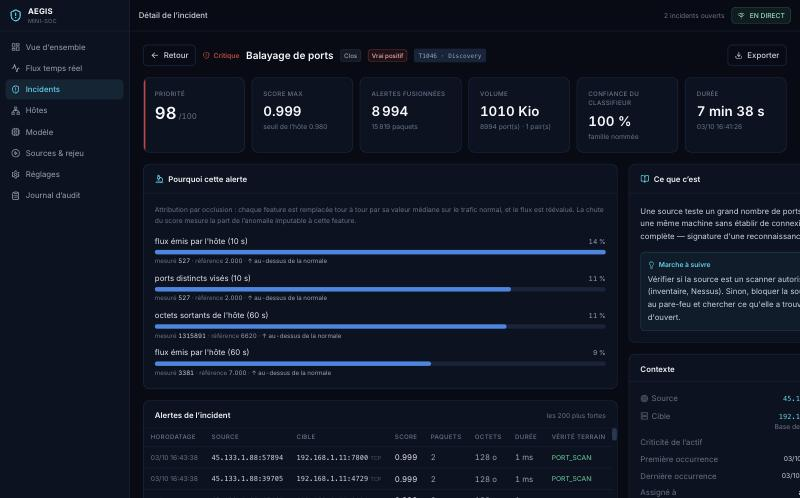
\includegraphics[width=0.98\linewidth]{../docs/screenshots/05-incident-explication.jpg}
\caption{Détail d'un incident. Le panneau \og{}Pourquoi cette alerte\fg{} donne les caractéristiques
responsables, avec la valeur mesurée et la valeur de référence.}
\end{figure}

\clearpage

\begin{figure}[h]\centering
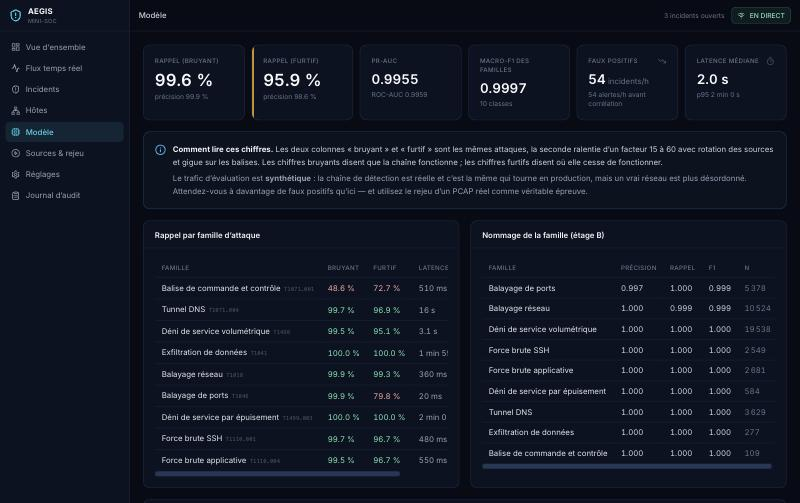
\includegraphics[width=0.98\linewidth]{../docs/screenshots/08-modele-metriques.jpg}
\caption{Écran Modèle : les deux colonnes bruyant et furtif, et le rappel par famille, affichés dans
le produit lui-même.}
\end{figure}

Huit écrans : vue d'ensemble, flux temps réel, file d'incidents, détail d'un incident, hôtes,
modèle, sources et rejeu, réglages et journal d'audit. Trois rôles sont vérifiés côté serveur :
lecteur, analyste et administrateur.

L'interface est écrite en TypeScript strict. Les couleurs des graphiques ont été validées par un
contrôle de lisibilité pour déficience de vision des couleurs plutôt que choisies à l'\oe{}il :
l'application n'emploie que deux couleurs de série, et la gravité, qui relève du statut et non de la
série, est toujours accompagnée d'une icône et d'un libellé --- le rouge, l'orange et le jaune sont
voisins sur la roue chromatique et ne peuvent pas porter seuls l'information.

%================================================================ 6
\section{Résultats}

\begin{table}[h]\centering\small
\begin{tabularx}{\linewidth}{@{}X r r@{}}
\toprule
\textbf{Mesure} & \textbf{Attaques bruyantes} & \textbf{Attaques furtives} \\
\midrule
Rappel & \textbf{99,56\%} & \textbf{95,94\%} \\
Précision & 99,89\% & 98,57\% \\
PR-AUC & 0,9955 & 0,9373 \\
Latence médiane de détection & 2,0 s & 6,0 s \\
\bottomrule
\end{tabularx}
\caption{Point de fonctionnement, mesuré en rejouant les captures de test dans le moteur réel.}
\end{table}

À quoi s'ajoutent \mesure{54 incidents de faux positifs par heure} sur du trafic ne contenant aucune
attaque, un macro-F1 de 0,9997 pour le nommage de la famille, et un débit d'environ 30\,000 paquets
par seconde en mono-processus.

\subsection*{Pourquoi deux colonnes}

Les variantes dites furtives sont les mêmes attaques ralenties d'un facteur quinze à soixante, avec
rotation des adresses sources, variation des tailles de requête et gigue de 25\% sur les balises.
Les chiffres bruyants établissent que la chaîne fonctionne ; les chiffres furtifs indiquent où elle
cesse de fonctionner. Publier les seconds est ce qui distingue une mesure d'une démonstration.

\subsection*{Le résultat le plus instructif}

Le rappel sur la balise de commande et contrôle plafonne à \mesure{48,6\%}. Ce chiffre est publié au
même titre que les autres, et c'est le plus riche d'enseignement du tableau.

Une balise émet peu : quelques centaines d'octets toutes les dizaines de secondes, poignée de main
complète, vers un port banal. Pris isolément, chacun de ses flux ressemble à une requête web
ordinaire --- c'est exactement l'effet recherché par un implant. Seule la périodicité la trahit, et
cette régularité n'apparaît qu'après plusieurs contacts, donc après un délai pendant lequel la
détection reste muette.

\subsection*{Le protocole de mesure}

\begin{enumerate}
\item L'étage A n'est entraîné que sur du trafic bénin : il ne voit jamais d'attaque.
\item La séparation entre entraînement et test se fait \textbf{par capture}, jamais par ligne. Des
flux issus d'une même rafale d'attaque sont fortement corrélés ; un découpage aléatoire produirait
les 99,9\% illusoires dont ce type de projet est coutumier.
\item Le point de fonctionnement est obtenu en rejouant les captures de test \textbf{dans le moteur
réel}, seuils adaptatifs compris, préchauffés sur une capture bénigne comme le serait une sonde
venant d'être déployée.
\item Les faux positifs sont mesurés sur des captures \textbf{sans aucune attaque} : la précision
calculée sur une capture riche en attaques flatte n'importe quel détecteur.
\item La latence est comptée du début de la fenêtre d'attaque jusqu'à la première alerte,
\textbf{délai d'export des flux inclus}, parce que ce délai est réel.
\end{enumerate}

\subsection*{Une nuance sur la précision}

La précision au niveau des flux atteint 99,89\%, tandis que la précision au niveau des
\emph{incidents}, telle que jugée par les analystes dans l'interface, tourne autour de 76\%. Ce
n'est pas une contradiction : un faux positif ne fusionne jamais, il constitue son propre incident,
alors qu'une véritable attaque fusionne des milliers d'alertes en une seule ligne. Le tableau de
bord affiche la valeur jugée par l'analyste, parce que c'est elle qui décrit la charge de travail
réelle.

%================================================================ 7
\section{Difficultés rencontrées}

\begin{description}[leftmargin=0pt,style=nextline,itemsep=4pt]
\item[Une statistique robuste ne l'est que pour la distribution qu'elle suppose.] L'application de
\texttt{médiane + k·MAD} à des percentiles saturait le seuil au plafond pour tous les hôtes. Le
rappel était tombé à 14\% sans qu'aucune métrique de classement ne le signale : le PR-AUC restait à
0,993, puisque le modèle classait correctement et que seul le point de fonctionnement était absurde.

\item[Une optimisation peut s'effondrer là où elle est le plus nécessaire.] Le parcours des flux
actifs à chaque paquet tenait très bien en trafic ordinaire, et cédait pendant une inondation ou un
slowloris --- c'est-à-dire exactement quand le détecteur doit tenir.

\item[Une latence se mesure au moment où l'information devient disponible.] Elle était comptée sur
le dernier paquet du flux, non sur son export, et ignorait donc le délai propre à une détection par
flux. Le chiffre publié est passé de 0,67 à 3,0 secondes : le système n'a pas ralenti, la mesure est
devenue vraie.

\item[Un générateur qui ne sort jamais de la mémoire peut produire l'impossible.] Les sessions SSH
tiraient deux nombres aléatoires indépendants, l'un pour la taille de trame annoncée, l'autre pour
la longueur de la charge utile : elles émettaient des trames déclarant 206 octets tout en en
transportant 256. Personne ne s'en plaignait jusqu'à ce qu'il faille les écrire dans un vrai fichier
pcap.

\item[\texttt{os.urandom} casse la reproductibilité sans prévenir.] Les charges utiles chiffrées en
provenaient : deux exécutions avec la même graine produisaient les mêmes flux avec des octets
différents, ce qui rendait impossible toute vérification du rejeu.

\item[SQLAlchemy applique les valeurs par défaut à l'INSERT,] pas à la construction de l'objet. Une
ligne fraîchement créée contenait encore \texttt{None}, et la première incrémentation tuait la tâche
d'ingestion --- silencieusement, puisque l'exception était rangée dans l'état du pipeline plutôt que
remontée.

\item[Un graphique collé à son plafond apprend à l'opérateur à ne plus le regarder.] Le score
maximum par seconde dépassait 0,95 dans 58\% des secondes sans qu'il se passe quoi que ce soit :
c'est une conséquence mécanique de la calibration par percentiles, et c'est la moyenne qu'il fallait
tracer.
\end{description}

%================================================================ 8
\section{Limites assumées et orientations futures}

\textbf{Le trafic d'évaluation est synthétique.} La chaîne de détection est réelle et c'est
exactement la même qui fonctionne en production ; le trafic qui l'alimente est généré. Un réseau
réel est plus désordonné, et produira davantage de faux positifs. Le rejeu d'une capture réelle est
la véritable épreuve, et le système est construit pour.

\textbf{Les familles sont séparables par construction}, ce qui explique le macro-F1 très élevé de
l'étage B sur les variantes bruyantes.

\textbf{La capture d'une interface réelle n'a jamais été exercée} : le code existe et sa gestion de
contre-pression est testée, mais l'accès aux périphériques BPF exige les privilèges administrateur.

\textbf{La détection est par flux, non par paquet} : la latence inclut le délai d'export. Le système
ne comporte qu'une sonde, sans agrégation multi-capteurs, et n'inspecte pas la couche applicative.

Les suites naturelles, par ordre de valeur : un rejeu validé sur le jeu public CIC-IDS2017 avec ses
étiquettes officielles, ce qui permettrait la comparaison avec la littérature ; le ré-entraînement
sur les verdicts d'analystes, déjà enregistrés en base mais non encore exploités ; un suivi de
dérive entre la distribution d'entraînement et le trafic du jour ; une réponse automatique en mode
simulation par défaut ; enfin l'agrégation de plusieurs sondes vers un corrélateur central.

%================================================================ 9
\section{Conclusion}

Le projet livre une chaîne de détection complète et mesurée : 52 caractéristiques extraites de flux
assemblés à 30\,000 paquets par seconde, un modèle à deux étages dont le score est interprétable,
des seuils qui s'adaptent à chaque machine, une corrélation qui ramène des milliers d'alertes à une
ligne de travail, et une interface de triage traçable. Quatre-vingt-quatorze tests couvrent le
moteur, la détection, l'API et l'aller-retour des captures.

L'objectif n'était pas d'obtenir un score élevé sur un jeu de données public, mais de construire
l'ensemble de la chaîne et de la mesurer honnêtement --- y compris là où elle échoue, ce que le
rappel de 48,6\% sur la balise de commande et contrôle illustre mieux que n'importe quel autre
chiffre du rapport.

\end{document}
